%!TEX root = ../main.tex

\chapter{Evaluation}

\label{Chapter4-evaluation}

% TODO write some intro here

\section{Parameters}

Each of our implemented key-value stores is instantiated with a set of parameters. In Chapter \ref{Chapter3-implementation} we explained what each parameter represents, but to be able to understand the trade-offs among them, and how various settings of them influence the behavior of the respective engine, it is important to explore them visually.

In this section, the experiments performed aim to highlight qualitatively the effect of each parameter and do not constitute stress tests.

For the following demonstrations, we use by default - unless explicitly stated otherwise - the following settings: The randomly generated keys and values have length 4 bytes, the sets of available keys and values have cardinality $10^3$ each, the distribution of picking keys and values from the sets is uniform, the input write and read throughput are $10^3$ writes and $10^3$ reads per second respectively, and for latency measurements that are sampled (to calculate the 50th and the 95th percentile), the number of samples is 10. Also, for the LSM-Tree we use \verb"max_runs_per_level="3, \verb"memtable_bytes_limit="$10^3$, \verb"density_factor="10, and for the parameters of HybridLog we use \verb"mem_segment_len="$10^4$, \verb"ro_lag_interval="$10^3$, \verb"flush_interval="$10^3$, and \verb"compaction_enabled=False".

\subsection{LSM-Tree}

\subsubsection{Max Runs per Level}

The first parameter of the LSM-Tree is \verb"max_runs_per_level". This controls the maximum amount of runs allowed in a level. As explained in Chapter \ref{Chapter3-implementation}, as the number of runs per level increases, a log-structured database becomes write-optimized, and when it is kept close to 1, the database is optimized for reads. In figure \ref{fig:max-runs-per-level} we demonstrate this behavior:

\begin{figure}[h]
    \begin{subfigure}{.5\textwidth}
        \centering
        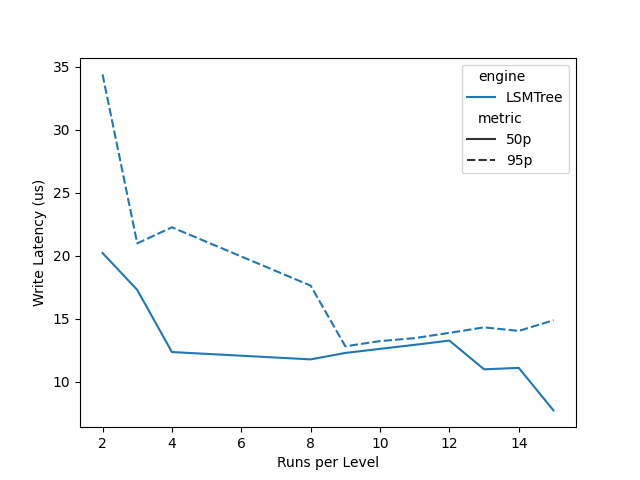
\includegraphics[width=1.1\linewidth]{max_runs_per_level_write.png}
    \end{subfigure}
    \begin{subfigure}{.5\textwidth}
        \centering
        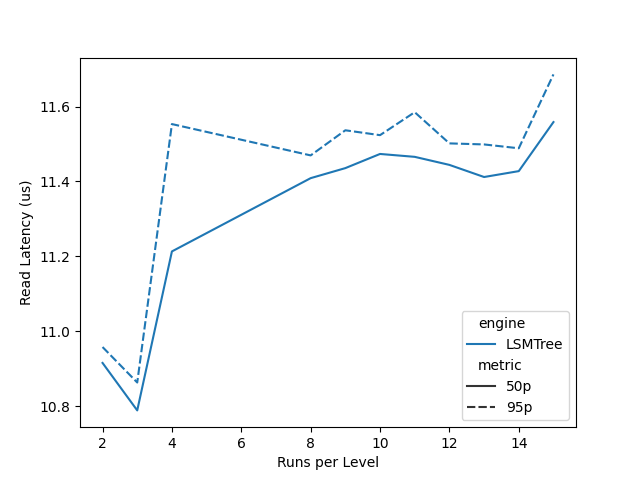
\includegraphics[width=1.1\linewidth]{max_runs_per_level_read.png}
    \end{subfigure}
    \caption{Latency vs Max Runs per Level.}
    \label{fig:max-runs-per-level}
\end{figure}

Clearly, the write latency drops, when \verb"max_runs_per_level" increases, and the read latency is low when the parameter is relatively small.

The LSM-Tree behaves as expected due to the following reasons: when the number of runs per level increases, the log-structuring scheme degrades into a large fragmented log spread over several smaller logs with infrequent merges. This essentially becomes a large log, enabling the maximum writing speed. However, at the same time, accessing a key requires searching through multiple runs per level, leading to slower reads.

This parameter is central, and relevant not only to the LSM-Tree but to the other two log-structured engines, HybridLog and AppendLog. More specifically, the effect on the write latency on these two is the same, but not quite so for the read latency. Because of the fundamental difference in indexing (the latter two use in-memory hash-based indices that point directly to files and offsets), the read latencies are not affected. One needs to just keep the parameter ``balanced'' enough so that then merges are not very large and infrequent, which would impact the overall performance of the stores.

\subsubsection{Density Factor}
The \verb"density_factor", as explained in section \ref{subsection-lsm-design}, controls the width of gaps between the fence pointers of the LSM-Tree.

\begin{figure}[h]
    \begin{subfigure}{.5\textwidth}
        \centering
        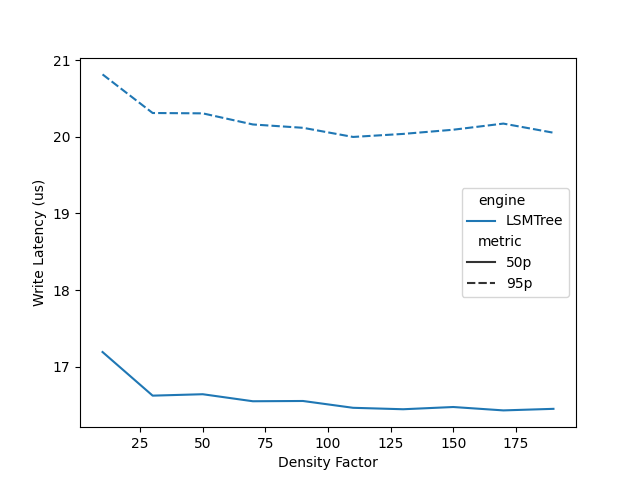
\includegraphics[width=1.1\linewidth]{density_factor_write.png}
    \end{subfigure}
    \begin{subfigure}{.5\textwidth}
        \centering
        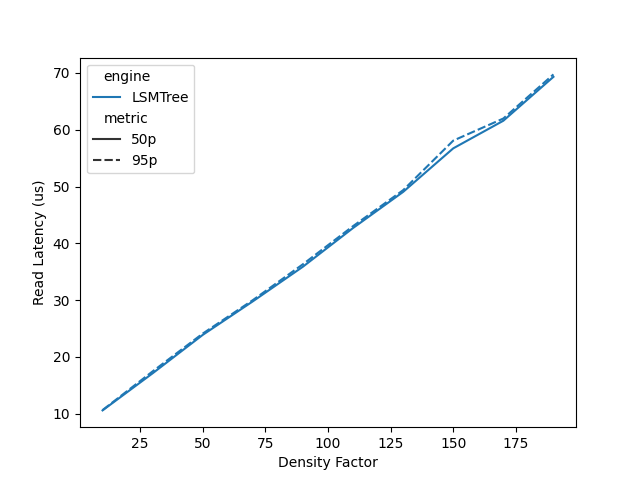
\includegraphics[width=1.1\linewidth]{density_factor_read.png}
    \end{subfigure}
    \caption{Latency vs Density Factor.}
    \label{fig:density_factor_write_read}
\end{figure}

\begin{figure}[h]
    \begin{subfigure}{.5\textwidth}
        \centering
        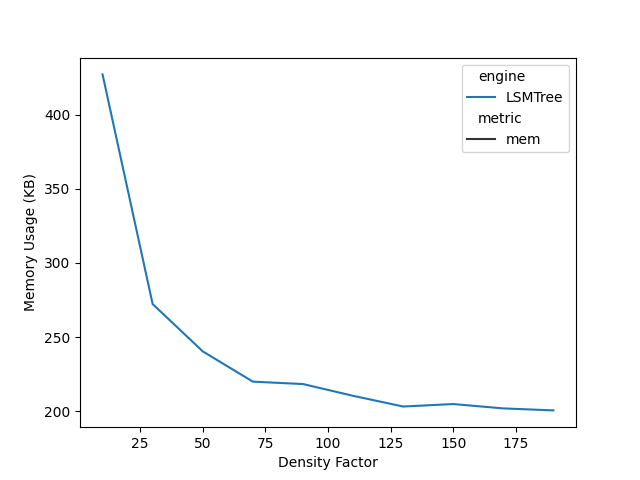
\includegraphics[width=1.1\linewidth]{density_factor_mem.png}
    \end{subfigure}
    \begin{subfigure}{.5\textwidth}
        \centering
        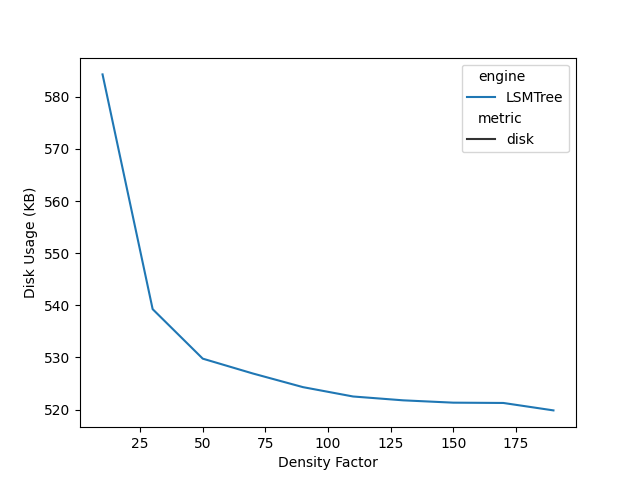
\includegraphics[width=1.1\linewidth]{density_factor_disk.png}
    \end{subfigure}
    \caption{Memory and Disk Usage vs Density Factor.}
    \label{fig:density_factor_mem_disk}
\end{figure}

In figure \ref{fig:density_factor_write_read} we observe the following: as the density factor increases, the writes remain virtually unaffected, and reads become drastically slower. This is because the LSM-Tree, when the density factor is high and therefore the gaps within the offsets are large, has to go through more bytes in the file to find the requested key, which slows down the reads.

However, there is an obvious tension here: we cannot keep the density factor too small, because that would result in higher memory and disk usage, as demonstrated in figure \ref{fig:density_factor_mem_disk}.

\subsubsection{Memtable Size}

The size of the LSM-Tree's memtable, controlled by the \verb"memtable_bytes_limit", is the amount of bytes the in-memory structure can hold before it flushes to disk.

\begin{figure}[h]
    \begin{subfigure}{.5\textwidth}
        \centering
        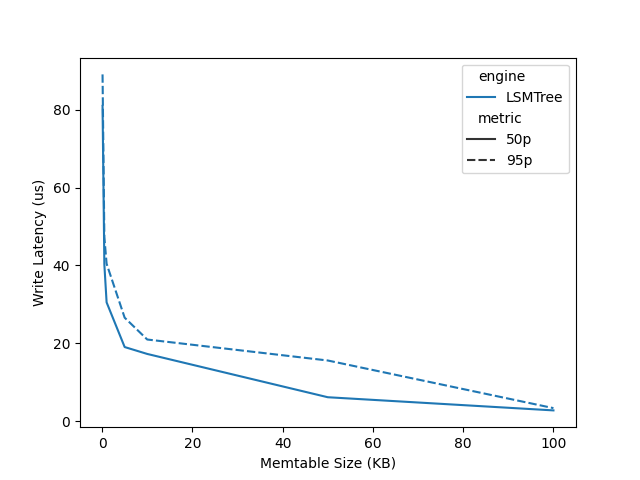
\includegraphics[width=1.1\linewidth]{memtable_bytes_limit_write.png}
    \end{subfigure}
    \begin{subfigure}{.5\textwidth}
        \centering
        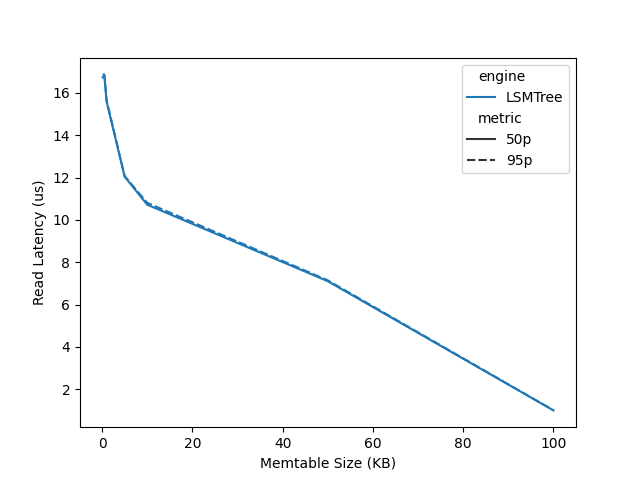
\includegraphics[width=1.1\linewidth]{memtable_bytes_limit_read.png}
    \end{subfigure}
    \caption{Latency vs Memtable Size.}
    \label{fig:memtable-bytes-limit-write-read}
\end{figure}

\begin{figure}[h]
    \centering
    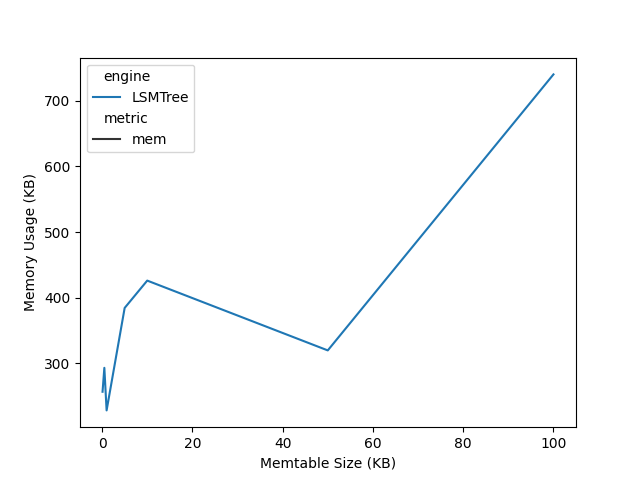
\includegraphics[width=0.6\textwidth]{memtable_bytes_limit_mem.png}
    \caption{Memory Usage vs Memtable Size}
    \label{fig:memtable_bytes_limit_mem}
\end{figure}

In figure \ref{fig:memtable-bytes-limit-write-read} we notice that as the size of the memtable increases, the latency of both the writes and reads drops. This is expected, as with bigger memtables, the probability of accessing a key without the need to reach to the disk is higher. However, the memory usage obviously goes up, as seen in figure \ref{fig:memtable_bytes_limit_mem}, and thus we cannot keep this parameter too large.

\subsection{HybridLog}

\subsubsection{Memory Segment Size}

Besides the indices, HybridLog also keeps a memory segment in memory, which is essentially a ring buffer. The parameter \verb"mem_segment_len" controls the size of this segment. In figure \ref{fig:mem_segment_len_write_read} we see its influence in the latencies of the writes and the reads, and in figure \ref{fig:mem_segment_len_mem.png} we see the memory usage.

\begin{figure}[h]
    \begin{subfigure}{.5\textwidth}
        \centering
        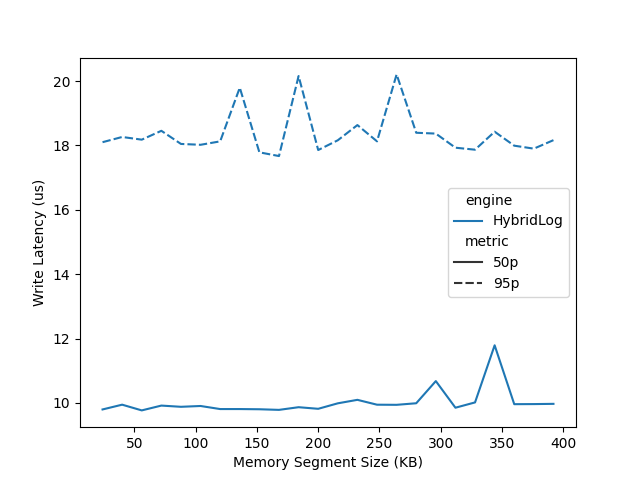
\includegraphics[width=1.1\linewidth]{mem_segment_len_write.png}
    \end{subfigure}
    \begin{subfigure}{.5\textwidth}
        \centering
        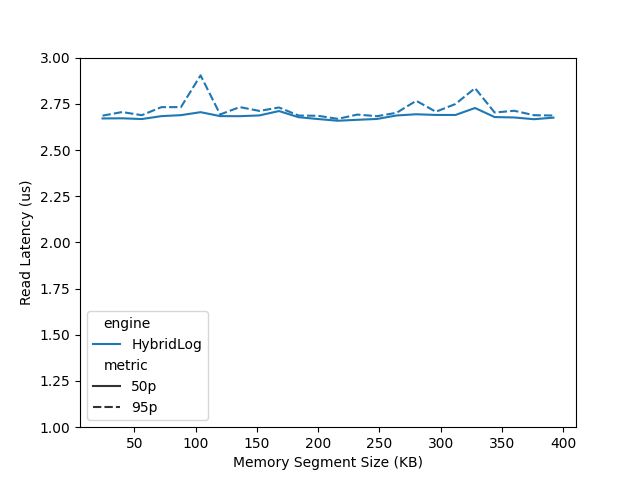
\includegraphics[width=1.1\linewidth]{mem_segment_len_read.png}
    \end{subfigure}
    \caption{Latency vs Memory Segment Length.}
    \label{fig:mem_segment_len_write_read}
\end{figure}


\begin{figure}[h]
    \centering
    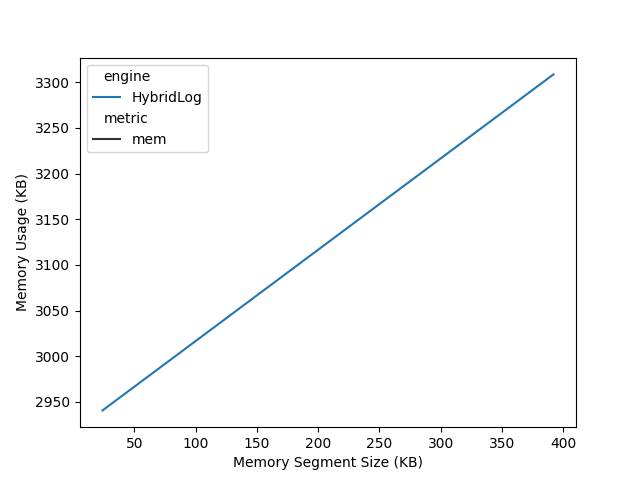
\includegraphics[width=0.6\textwidth]{mem_segment_len_mem.png}
    \caption{Memory Usage vs Memory Segment Size}
    \label{fig:mem_segment_len_mem.png}
\end{figure}

As expected, the size of the in-memory segment is irrelevant to the speed of both writes and reads, while it directly affects the memory used by the engine. It is irrelevant to the latencies because, as we will see later, it is the \verb"ro_lag_interval" which actually matters.

Hence, it is important that we keep this parameter as low as possible. Since it must always hold that the size of the memory segment is larger than the sum of the sizes of the sub-segments defined by \verb"ro_lag_interval" and \verb"flush_interval", this parameter should ideally be set a value slightly larger than the sum of these two intervals.

\subsubsection{Read-only Segment Size}

The read-only segment size is controlled via the value of \verb"ro_lag_interval". Contrary to the memory segment size, this is the parameter which actually influences directly the probability of an in-memory hit of a key lookup, and thus the cache-like behavior of the whole memory segment.

If this value is big, we expect many in-memory hits, therefore better performance for both writes and reads. This is exactly what we observe in figure \ref{fig:ro_lag_interval}.

\begin{figure}[h]
    \begin{subfigure}{.5\textwidth}
        \centering
        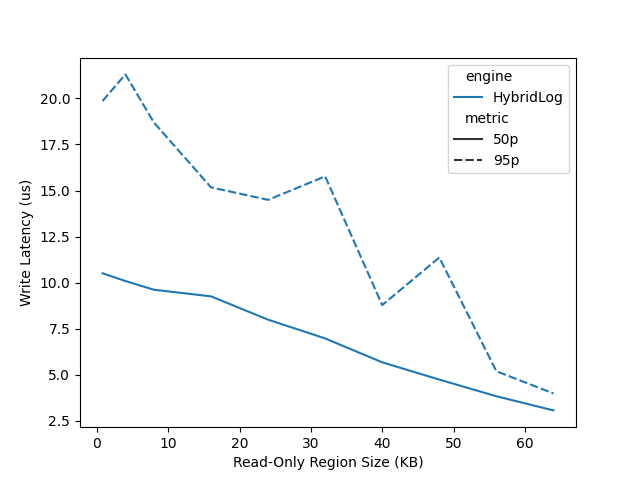
\includegraphics[width=1.1\linewidth]{ro_lag_interval_write.png}
    \end{subfigure}
    \begin{subfigure}{.5\textwidth}
        \centering
        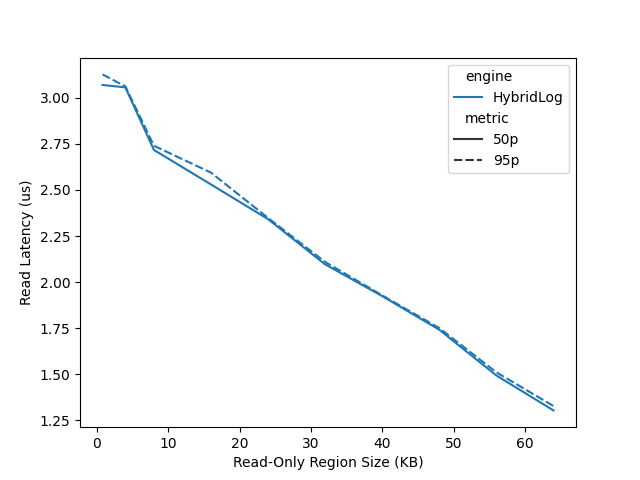
\includegraphics[width=1.1\linewidth]{ro_lag_interval_read.png}
    \end{subfigure}
    \caption{Latency vs Read-only Segment Size.}
    \label{fig:ro_lag_interval}
\end{figure}

\subsubsection{Flush Segment Size}

The flush segment, whose size is adjusted via the \verb"flush_interval" parameter, contains read-only entries that are ready to be flushed to disk. The bigger the segment, the less the probability for disk access and therefore the higher the performance of the key-value store. This is evident in figure \ref{fig:flush_interval_write_read}. The obvious trade-off present here, is that if this value is set to be large, we require a larger memory segment size, which will use more memory.


Additionally, it is crucial to ensure that the value is not set too low. If it is set too low, it may impede the speedup of performance from large flushes to disk, which occur sequentially and are therefore fast. Furthermore, setting the value too low may result in numerous small logs that require frequent merges, thus adversely impacting performance. This phenomenon is also illustrated in the same figure \ref{fig:flush_interval_write_read}.

\begin{figure}[h]
    \begin{subfigure}{.5\textwidth}
        \centering
        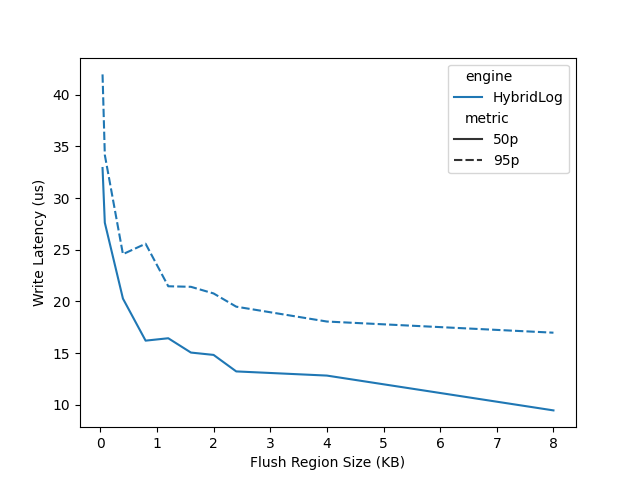
\includegraphics[width=1.1\linewidth]{flush_interval_write.png}
    \end{subfigure}
    \begin{subfigure}{.5\textwidth}
        \centering
        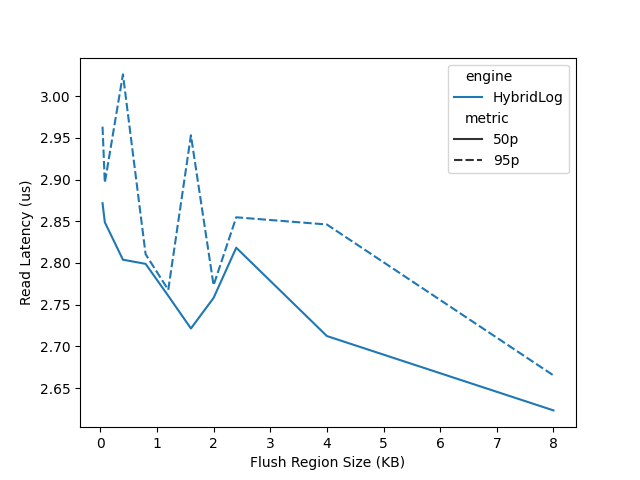
\includegraphics[width=1.1\linewidth]{flush_interval_read.png}
    \end{subfigure}
    \caption{Latency vs Flush Segment Size.}
    \label{fig:flush_interval_write_read}
\end{figure}

\subsubsection{Compaction}

Regarding compaction, one may wonder if it could offer some speedup in practice, since it could be the case that its potential benefit is implicitly provided during merging already, and the system is just wasting time doing extra unnecessary work.

\begin{figure}[h]
    \centering
    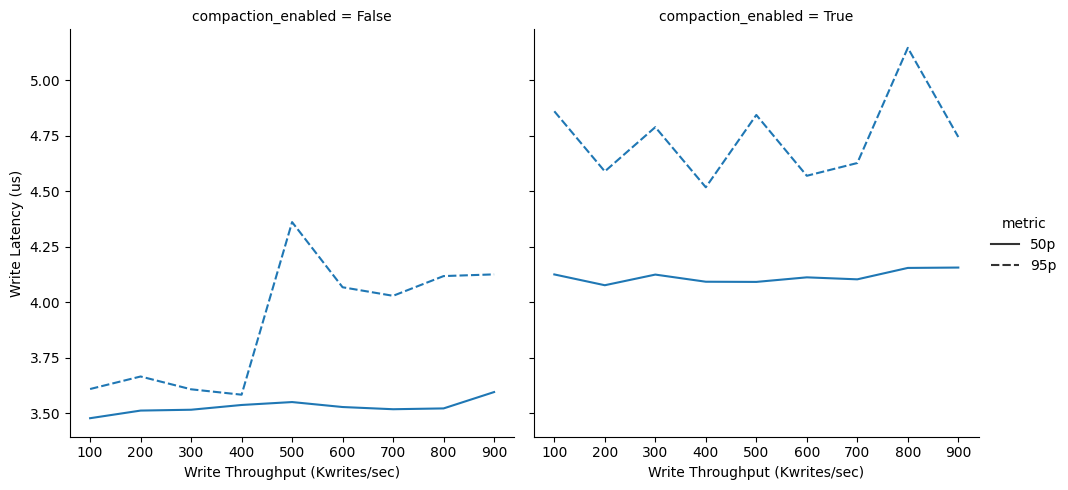
\includegraphics[width=1\textwidth]{compaction_write.png}
    \caption{Write Latency vs Throughput, with Compaction disabled (left) and enabled (right).}
    \label{fig:compaction-write}
\end{figure}

\begin{figure}[h]
    \centering
    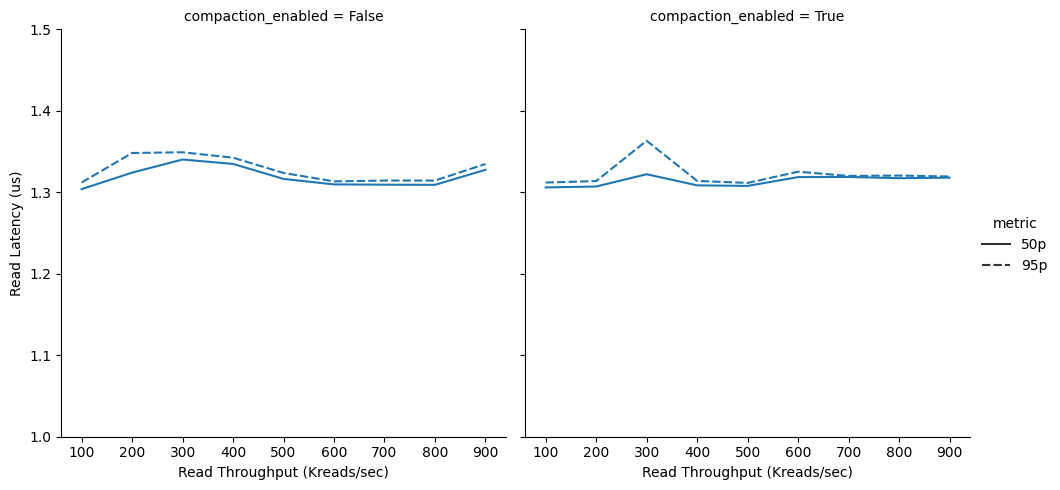
\includegraphics[width=1\textwidth]{compaction_read.png}
    \caption{Read Latency vs Throughput, with Compaction disabled (left) and enabled (right).}
    \label{fig:compaction_read}
\end{figure}

From the experiment results in figures \ref{fig:compaction-write} and \ref{fig:compaction_read} it seems that this is exactly the case. Compaction offers no advantage for reads (which was expected, since file access is still the same), but also neither for writes, which are in fact impaired, as compaction introduces a significant overhead. Therefore, compaction should be avoided in log-structuring.

\subsection{AppendLog}

In AppendLog we only have one tunable parameter, the threshold value, which is the maximum amount of bytes we can write to a runfile before closing it and starting the next one.

This parameter is similar to the \verb"flush_interval" parameter of the HybridLog. When it is too low, frequent merges hinder the write performance, and as it increases, writes on average become faster (because the runfile becomes essentially a large append-only log). However, if the threshold is too high, the files become large and the merges infrequent and cumbersome, which explains the widening of the gap between the 50p and 95p lines in the write latencies in figure \ref{fig:threshold_write_read}. As for the reads, they are not significantly affected, as expected.

\subsubsection{Threshold}

\begin{figure}[h]
    \begin{subfigure}{.5\textwidth}
        \centering
        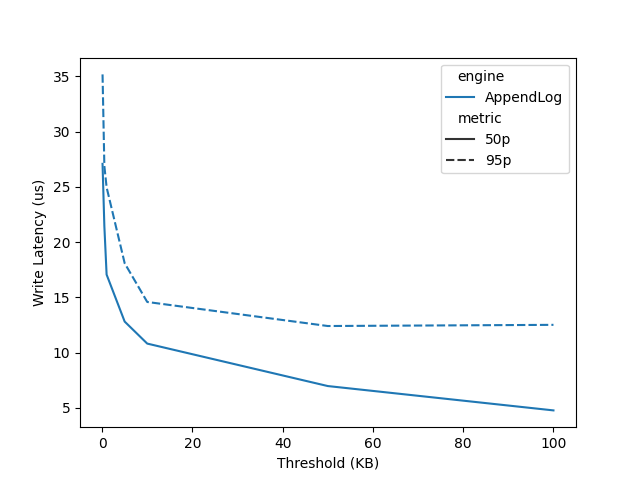
\includegraphics[width=1.1\linewidth]{threshold_write.png}
    \end{subfigure}
    \begin{subfigure}{.5\textwidth}
        \centering
        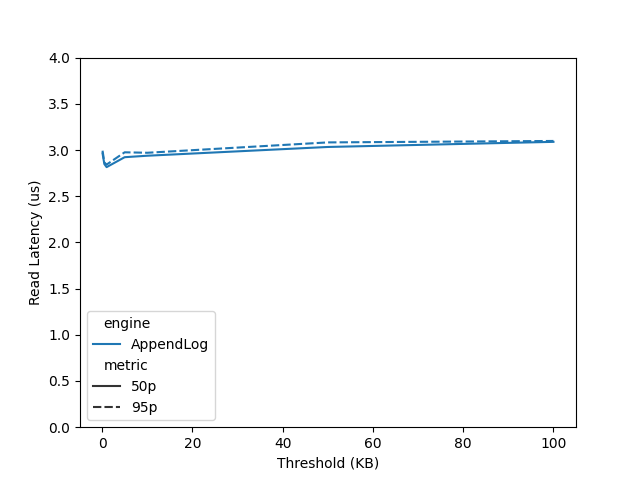
\includegraphics[width=1.1\linewidth]{threshold_read.png}
    \end{subfigure}
    \caption{Latency vs Threshold.}
    \label{fig:threshold_write_read}
\end{figure}

\section{Comparison}

In this section we proceed to compare the engines on their performances when executing the same task with similar parameters. For the following experiments, we use the following parameters: Key and value lengths of 5 bytes each (so 10-byte key-value pairs), $10^5$ unique keys and values, and 10 samples per average latency measurement for the percentiles. Also, for all engines we use \verb"max_runs_per_level="10, for the LSM-Tree \verb"density_factor="10 and \verb"memtable_bytes_limit="100K, for the HybridLog \verb"mem_segment_len="210K, \verb"ro_lag_interval="10K, \verb"flush_interval="10K, and for the AppendLog \verb"threshold="100K.

The above settings lead to almost equally sized files on disk, and use the same configurable memory, so the comparison is fair.

\subsection{Write Latencies}

In figure \ref{fig:comparison-write} we observe the write latencies of each engine as we increase the input throughput. When choosing keys uniformly, HybridLog and AppendLog are significantly faster than the LSM-Tree. This can be attributed to the fast (amortized $\mathcal{O}(1)$) hash-based indexing of those engines, versus the LSM-Tree's memtable's data structure, which has an insert complexity of $\mathcal{O}(\log{}(n))$. This is also the reason that when we use a state with a size that fits the in-memory structures and therefore does not need to ``spill'' to disk, the HybridLog still performs faster, as can be seen in figure \ref{fig:comparison-write-fit-mem}.

When we choose keys using a Zipfian distribution instead, some keys are accessed compared to the Uniform distribution, the LSM-Tree and the HybridLog become faster than earlier, because the Zipfian distribution allows them to better leverage their in-memory buffering structures before flushing, thus reducing I/O operations, and the AppendLog becomes slower, because it lacks any similar buffering method to take advantage of the Zipfian distribution. Among them, the HybridLog is clearly the fastest, precisely because its memory segment with its fast in-place updates of recently written records exploits the Zipfian distribution best.


\begin{figure}[h]
    \begin{subfigure}{.5\textwidth}
        \centering
        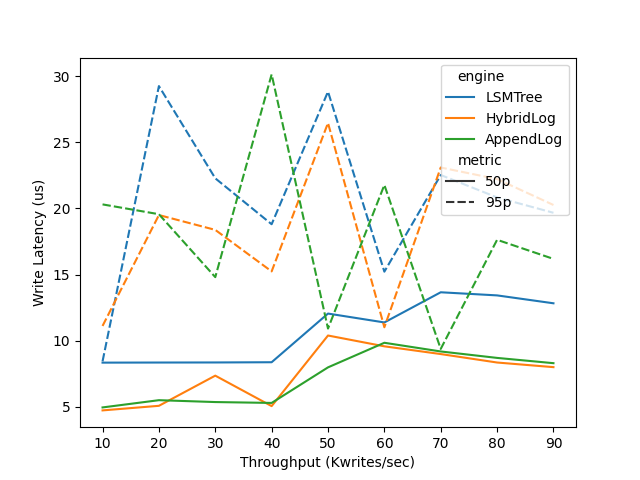
\includegraphics[width=1.1\linewidth]{write-throughput.png}
        \caption{Uniform distribution}
    \end{subfigure}
    \begin{subfigure}{.5\textwidth}
        \centering
        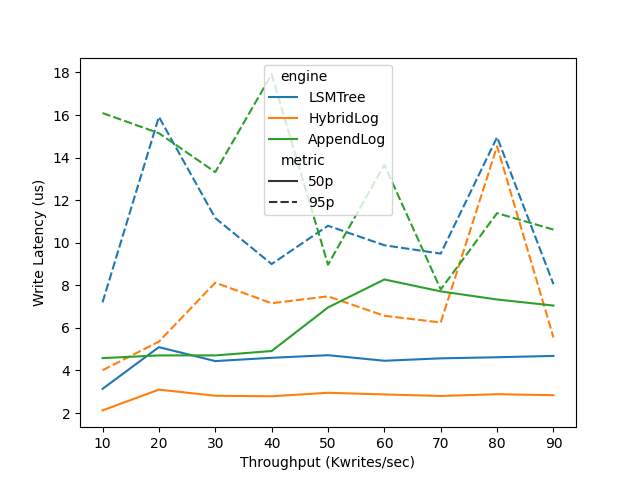
\includegraphics[width=1.1\linewidth]{write-throughput-zipfian.png}
        \caption{Zipfian distribution}
    \end{subfigure}
    \caption{Latency vs Max Runs per Level.}
    \label{fig:comparison-write}
\end{figure}

\begin{figure}[h]
    \centering
    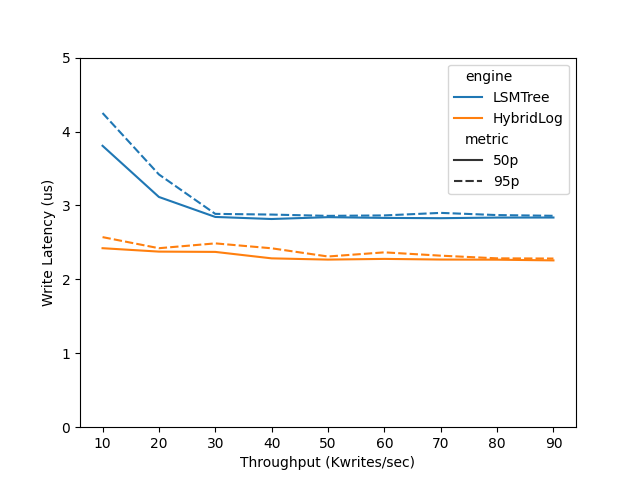
\includegraphics[width=0.6\textwidth]{write-throughput-fit-mem.png}
    \caption{Write Throughtput when data fits the memory}
    \label{fig:comparison-write-fit-mem}
\end{figure}

\subsection{Read Latencies}

Upon examining the latencies for the reads in figure \ref{fig:comparison-read-latencies}, it becomes clear that the HybridLog and AppendLog outperform the LSM-Tree by a large margin. This is because of their fast hash-based in-memory indices and minimal I/O.

\begin{figure}[h]
    \centering
    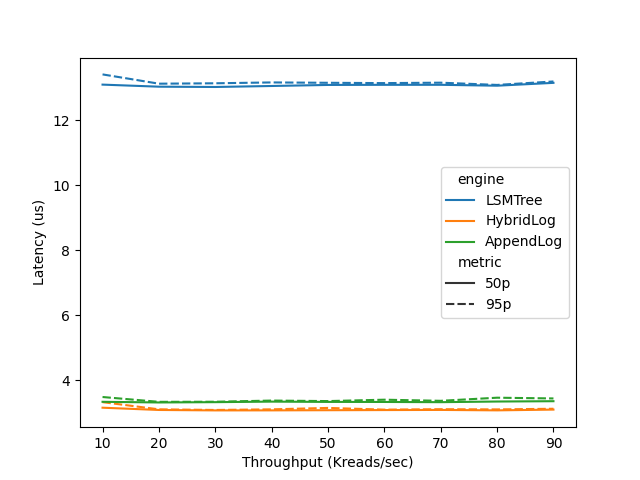
\includegraphics[width=0.6\textwidth]{read-throughput.png}
    \caption{Read Latencies}
    \label{fig:comparison-read-latencies}
\end{figure}

\subsection{Memory}

HybridLog's superiority as the fastest key-value store comes at the cost of high memory usage, as can be seen in figure \ref{fig:comparison-memory}. Indeed, it is the store with the most in-memory structures, including its main index. After that comes the AppendLog, which also keeps its index in memory. Finally, the LSM-Tree uses the least memory of all, making it ideal for low-memory environments (and also the cheaper option). The components requiring memory in the LSM-Tree are the Bloom filters and the fence pointers, which we keep in memory for fast access.

\begin{figure}[h]
    \centering
    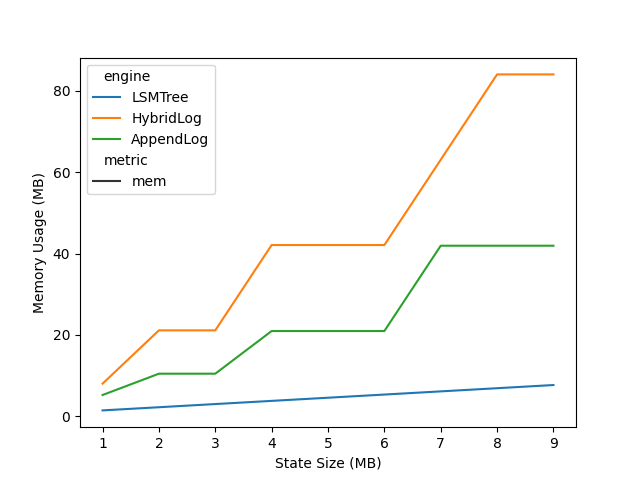
\includegraphics[width=0.6\textwidth]{mem.png}
    \caption{Memory Usage}
    \label{fig:comparison-memory}
\end{figure}

\section{Incremental Snapshotting}

This section focuses on evaluating the incremental snapshotting capabilities of the three log-structured engines. Towards this goal, to demonstrate the advantage of having incremental snapshots, we compare the LSM-Tree, HybridLog and AppendLog to ``MemOnly'', which is a naive implementation of a key-value store based on an entirely in-memory hosted HashMap that dumps its whole state to disk every time we want to take a snapshot of it.

We do two experiments. In the first, we iterate and write new key-value pairs, taking also a snapshot at the end of each iteration. In the second experiment, we first perform a large write-volume of 1GB, and then we write data in small increments on 1KB, taking a snapshot after each increment.

For both experiments, we use keys and values of 2 and 8 bytes respectively so that the available keys are no more than $2^{16}$ and therefore we will not need too much memory for the indices of HybridLog, AppendLog and MemOnly. Also, to simulate a snapshot over the network, we add an overhead of 1$\mu$s per byte (as if we had a network channel of 1MB/s). The settings for all engines are similar so that the comparison is as fair as possible.

The results of the first experiment are shown in figure \ref{fig:snapshot}. As expected, the naive MemOnly database dumps the whole state at every step, leading to a quadratic increase of the total time taken to take $n$ snapshots, while the other log-structured stores increase linearly. During each snapshotting step, they only dump the new inserts, except from a few cases when some merging takes place and have to push some larger files as well, but still, they perform better than MemOnly.

For the second experiment, where only updates take place, the results can be seen in figure \ref{fig:snapshot-static-state}. Again, as expected, the LSM-Tree, HybridLog and AppendLog only push the updates, while the MemOnly store pushes the whole state every time. By observing the cumulative graph, it is evident that the log-structured stores take snapshots more efficiently than the naive method.

\begin{figure}[h]
    \begin{subfigure}{.5\textwidth}
        \centering
        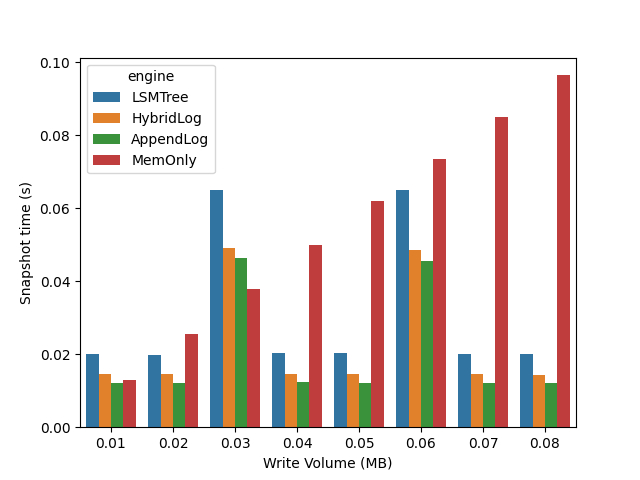
\includegraphics[width=1.1\linewidth]{snapshot.png}
        \caption{Discrete}
    \end{subfigure}
    \begin{subfigure}{.5\textwidth}
        \centering
        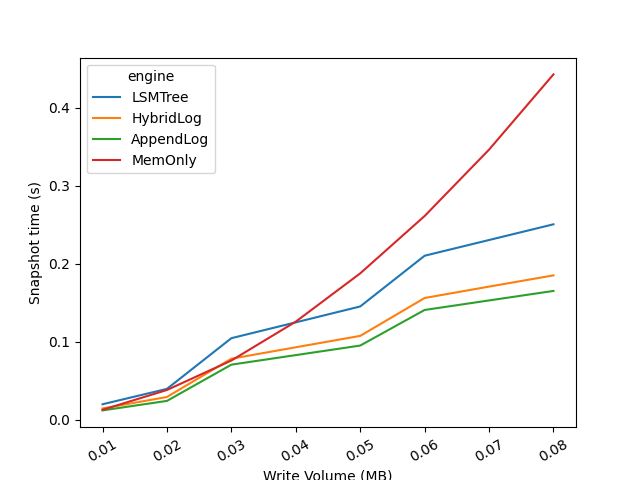
\includegraphics[width=1.1\linewidth]{snapshot-aggr.png}
        \caption{Cumulative}
    \end{subfigure}
    \caption{Snapshotting Time vs Write Volume, when we increase the state by inserting new records.}
    \label{fig:snapshot}
\end{figure}

\begin{figure}[h]
    \begin{subfigure}{.5\textwidth}
        \centering
        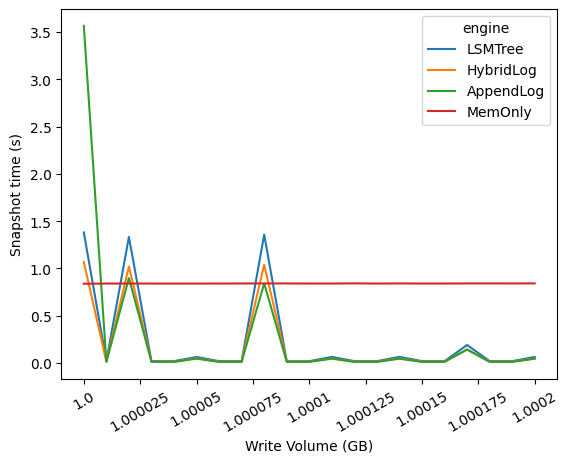
\includegraphics[width=1.1\linewidth]{snapshot-static-state.png}
        \caption{Discrete}
    \end{subfigure}
    \begin{subfigure}{.5\textwidth}
        \centering
        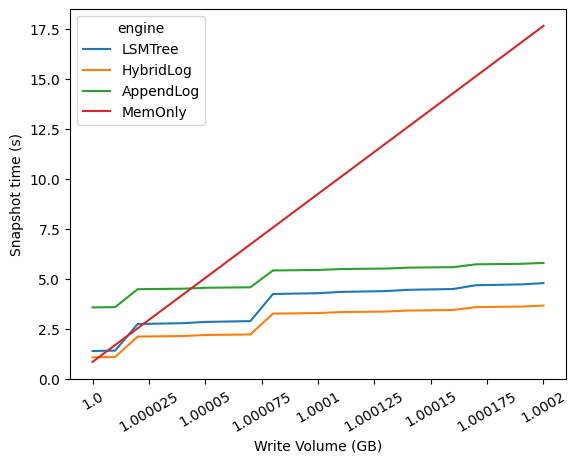
\includegraphics[width=1.1\linewidth]{snapshot-static-state-aggr.png}
        \caption{Cumulative}
    \end{subfigure}
    \caption{Snapshotting Time vs Write Volume, when state stays the same and we only update it.}
    \label{fig:snapshot-static-state}
\end{figure}

The important takeaway from these two experiments is that while the cumulative time of the naive snapshotting method increases quadratically at the worst case, the log-structured incremental methods increase linearly. This distinction can have significant ramifications in the performance of systems that keep large states.

% \section{Discussion}

% TODO table with advantages and disadvantages of each kvstore.

% LSM-Tree: all keys values on disk
% AppendLog: keys must fit mem
% HybridLog: keys must fit mem
% MemOnly: keys and values must fit mem

% HybridLog: fastest performance

% AppendLog: fastest snapshot

% LSM-Tree: fastest recovery, lowest memory

%lsm, append: they dont lose data
%hybrid log: may lose data
% although these are not that crucial for our case since we are manually snapshotting
